\documentclass[tikz]{standalone}
\usepackage{pgfplots}
\pgfplotsset{compat=1.18}

\begin{document}

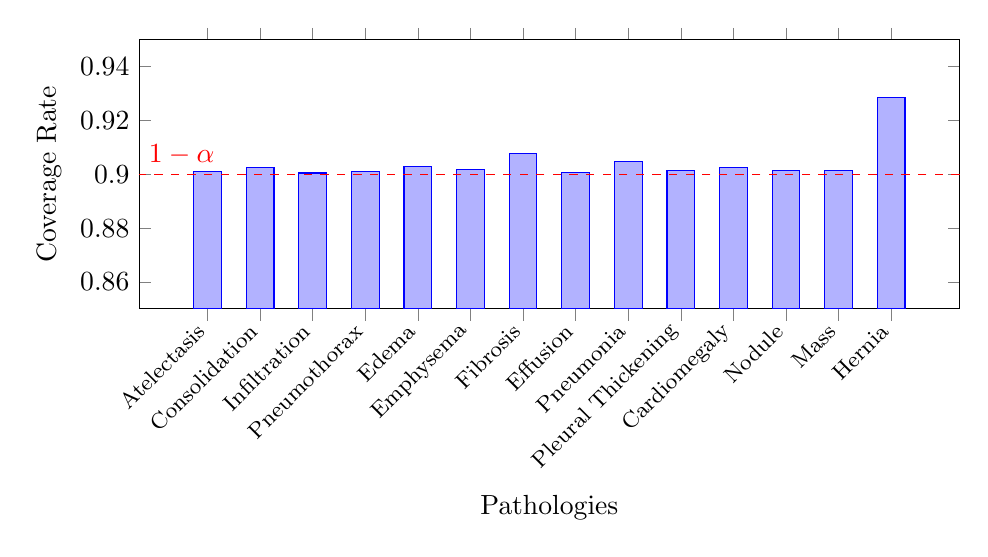
\begin{tikzpicture}
\begin{axis}[
    width=12cm,
    height=5cm,
    ybar,
    symbolic x coords={Atelectasis, Consolidation, Infiltration, Pneumothorax, Edema, Emphysema, Fibrosis, Effusion, Pneumonia, Pleural Thickening, Cardiomegaly, Nodule, Mass, Hernia},
    xtick=data,
    xticklabel style={
        font=\footnotesize,
        rotate=45,
        anchor=east
    },
    ylabel=Coverage Rate,
    ymin=0.85, ymax=0.95,
    xlabel={Pathologies},
    enlarge x limits=0.10,
    legend pos=north east,
]

\addplot coordinates {
    (Atelectasis, 0.9011)
    (Consolidation, 0.9026)
    (Infiltration, 0.9005)
    (Pneumothorax, 0.9011)
    (Edema, 0.9030)
    (Emphysema, 0.9018)
    (Fibrosis, 0.9078)
    (Effusion, 0.9006)
    (Pneumonia, 0.9048)
    (Pleural Thickening, 0.9013)
    (Cardiomegaly, 0.9025)
    (Nodule, 0.9013)
    (Mass, 0.9015)
    (Hernia, 0.9286)
};

\path (axis cs:{[normalized]1},0.9) coordinate (aux);
\end{axis}

\draw[red, dashed] (current axis.east|-aux) -- (current axis.west|-aux) node [above right] {\(1 - \alpha\)};
\end{tikzpicture}

\end{document}
